\documentclass{article}

% inputenc package, allows the user to input accented characters directly from the keyboard
\usepackage[utf8]{inputenc}

% The ti­tling pack­age pro­vides con­trol over the type­set­ting of the \maketi­tle com­mand and \thanks com­mands, and makes the \ti­tle, \au­thor and \date in­for­ma­tion per­ma­nently avail­able.
\usepackage{titling}

% graphicx package, useful for including eps and pdf graphics
% include graphics with the command \includegraphics
\usepackage{graphicx}

\appto\listoftables{\addtocontents{lot}{\protect\setcounter{tocdepth}{2}}}

% Tells latex that the images are kept in a folder named figures under the current directory. 
\graphicspath{ {figures/} }

% Package that makes it possible to place two images beside eachother.
\usepackage{subcaption}

% The package defins figures called SCfigure and SCtable (analogous to figure and table) to typeset caption sideways. Options include innercaption, outercaption, leftcaption and rightcaption.  IS THIS USED ANYWHERE?
\usepackage{sidecap}

% A pack­age pro­vid­ing an in­ter­face to sec­tion­ing com­mands for se­lec­tion from var­i­ous ti­tle styles. E.g., marginal ti­tles and to change the font of all head­ings with a sin­gle com­mand, also pro­vid­ing sim­ple one-step page styles. Also in­cludes a pack­age to change the page styles when there are floats in a page. You may as­sign head­ers/foot­ers to in­di­vid­ual floats, too.
\usepackage[compact,explicit]{titlesec}

% A companion for titlesec handling toc/lof/lot entries. 
\usepackage{titletoc}

% The package hyperref provides LaTeX the ability to create hyperlinks within the document.
\usepackage{hyperref}

% The todonotes package allows you to insert to{do items in your docu-ment. At any point in the document a list of all the inserted to{do items can be listed with the \listoftodos command
\usepackage{todonotes}

% Package is used for the tasks section //Nick
\usepackage{tabto}

\usepackage{mdwlist}


%KNORN
\usepackage{hyperref}
\hypersetup{colorlinks=true, linkcolor=blue, urlcolor=blue}
%\usepackage[usenames,dvipsnames,svgnames,table]{xcolor}
\definecolor{entityColor}{RGB}{0,100,200}
\definecolor{attributeColor}{RGB}{0,100,50}
\definecolor{relationColor}{RGB}{160,0,30}
\usepackage{listings}
\lstdefinestyle{reqT}{
  belowcaptionskip=1\baselineskip,
  breaklines=true,
  showstringspaces=false,
  basicstyle=\footnotesize\sffamily,
  emph={Ent,Meta,Item,Label,Section,Term,Actor,App,Component,Domain,Module,Product,Release,Resource,Risk,Service,Stakeholder,System,User,Class,Data,Input,Member,Output,Relationship,Design,Screen,MockUp,Function,Interface,Epic,Feature,Goal,Idea,Issue,Req,Ticket,WorkPackage,Breakpoint,Barrier,Quality,Target,Scenario,Task,Test,Story,UseCase,VariationPoint,Variant},
  emphstyle=\bfseries\color{entityColor},
  emph={[2]has,is,superOf,binds,deprecates,excludes,helps,hurts,impacts,implements,interactsWith,precedes,requires,relatesTo,verifies},
  emphstyle={[2]\bfseries\color{relationColor}},
  emph={[3]Attr,Code,Constraints,Comment,Deprecated,Example,Expectation,FileName,Gist,Image,Spec,Text,Title,Why,Benefit,Capacity,Cost,Damage,Frequency,Min,Max,Order,Prio,Probability,Profit,Value,Status},
  emphstyle={[3]\color{attributeColor}},  
}
\lstset{style=reqT}
%KNORN


\begin{document}
\todo{Det blir nått käbbel med raden som tar bort kraven från table of contents, kika sida 1 i förhandsgranskningen..}
%For the tasks, please do not alter/remove. 
\TabPositions{0.22\linewidth, 0.30\linewidth, 0.38\linewidth}

% Raden nedan ser till att nummret på en subsubsection kommer EFTER dess titel.
% Det är nuvarande lösning för att få kraven på formatet "Requirement 6.1.3"
\titleformat{\subsubsection}[runin]{\normalsize\bfseries}{}{0pt}{#1\quad\thesubsubsection}

\begin{titlepage}
    \noindent
    \textsc{Alexander Badju, Fredrik Helander, Jonathan Klingberg, Jonathan Knorn, David Lundberg, Niklas Sjöberg}\\ % Names of the authors of the document 
    \textsc{7/12-14}\\ % The date
    \vspace{10em}
    \begin{flushright}
    {\huge Software Requirements Specification R3}\\ % The document name
    {\large Group F - Steve's Angels} \\
    \par\end{flushright}\vskip 0.5em
\end{titlepage}

\begingroup
\hypersetup{linkcolor=black}
\tableofcontents
\thispagestyle{empty}
\endgroup
\newpage
\begingroup
\hypersetup{linkcolor=black}
\listoffigures
\thispagestyle{empty}
\endgroup
\newpage
\pagenumbering{arabic}

\section{Introduction}
Our company Steve's Angels have found out that car manufacturers have realized that self-driving cars will have an important role in the future transportation market. Although there are systems in place today, none of them are complete in terms of security and functionality. Car manufacturers are looking for a complete system solution that can be integrated into their cars and be implemented in actual traffic. Steve's Angels have come in contact with the car manufacturer LADA, who are currently losing market shares and are in desperate need for a new product that will challenge the market. 

\section{Summary}
The system merges several existing systems in a car making it self-driven. Since human lives are at stake, CRASH puts high demands on stability and reliability of the systems integrated with CRASH. CRASH must make sure the ride is safe at all costs.

\subsection{Stakeholders}
\noindent Inner stakeholders:
\begin{itemize}
\item \textbf{End user} - All users that interact with the system such as the car owner and passengers. The end users have demands on the system to be safe and easy to use.
\item \textbf{LADA} - Car manufacturer and key customer for the CRASH system. LADA has a considerable amount of demands, which the system must fulfill in order to meet their business goals. CRASH also integrates with their existing modules such as the control system and sensors.
\item \textbf{Steve's Angels} - The developers of the software requirement specification. They have demands such that the system solution described in the requirement specification is structured and well formed. They might want to sell their solution to other companies since LADA is only a key customer who helped form the requirements and Steve's Angels own the SRS.
\end{itemize}

\noindent Outer stakeholders:
\begin{itemize}
\item \textbf{Trafikverket} - Responsible for the long-term planning of infrastructure in Sweden. Can probably save money if the roads are used more efficiently. 
\item \textbf{Polismyndigheten} - The police is responsible for enforcing traffic regulations, and thus influenced by this product. With autonomous cars there will probably be less traffic offences, and thus they do not need to allocate as much resources in this area. 
\item \textbf{Swedish parliament} - The Parliament decides on all laws in Sweden, and a change in the law would be needed to allow driver-less technology.
\item \textbf{Swedish government} - The government enforces the laws that Parliament decides on, see above.
\item \textbf{Trafikanalys} - Provides policy makers with a basis for making decisions about transport policy.
\item \textbf{Transportstyrelsen} - Secure and environmental friendly transports.
\item \textbf{Insurance companies} - Cars without drivers, or with only passengers (the driver is seen as a passenger when the car is running automatically) poses new problems concerning insurance and liability in traffic.
\item \textbf{Lantmäteriet} - Develops maps of Sweden, which is needed for the positioning system to work.
\item \textbf{Sveriges Trafikskolors Riksförbund} - The Swedish organization for driving schools.
\end{itemize}

\subsection{Main goals}
The goal is to deliver an autonomous vehicle system. As the car manufacturing industry develops, it is of great importance to keep up with the latest progress in terms of technology. Introducing new technology to the market is one way to maintain or expand market shares. The system we develop is our answer to the current market situation.

The system must provide maximum traffic safety using the very latest achievements in the fields of navigation and anti-collision technology. This together with high passenger comfortability and excellent fuel economy will place CRASH ahead of its competition.

\subsection{Actors and their objectives}
The system has a large number of external actors, which communicates with the system in one way or another.
\newline




\noindent
\textbf{Traveler} A Traveler is a person who sits in the car and can interact with the system even though he does not have to be authenticated by the system.\\
\textbf{Passenger} A Passenger can unlock the car, press the emergency stop button and ride in the car alone.\\
\textbf{Driver} Can do anything that a passenger can.
The driver can also drive the car manually, handle the voice control as well as choosing the destination. \\
\textbf{Owner} Can do anything that a driver can. The owner also handles user management, in other words which users that are allowed to be drivers or passengers. \\
\textbf{Administrator} Can do anything that an owner can.
The administrator can change the system settings as well as general admin management \\
\todo{Vi säger att en admin kan ändra system settings, men har inga krav på dessa, ska vi ta bort det istället?}
\textbf{Control system} - A system that control the cars maneuvering components such as throttle and steering components. \\
\textbf{Weather forecast system} - A system that  provide weather forecasts that the car can download and use to warn about dangerous weather conditions along the current route.  \\
\textbf{Position data system} - A system where the car can upload its current position. Used by the owner to locate the cars position and follow it along its path.  \\
\textbf{Traffic information system} - A system that keeps track of the current traffic situation (e.g. accidents, queues etc). \\
\textbf{Surroundings sensory system} - A system that consists of several different sensors that senses the cars surroundings.  \\

\begin{figure}[htb]    
 \centering
  \includegraphics[width=0.9\textwidth]
    {"Context diagram v5".png}% bild på vårat context diagram
  \caption{Context diagram with actors and key components within the system.}
  \label{ContextDiagram}
\end{figure}
\todo{Måste uppdatera kontext till senaste och ändra Actors and objectives så att det stämmer överens}
\subsection{Terminology}
\textbf{The system} - The delivered product. When nothing else is stated, requirements are specified for autonomous driving mode.\\
\textbf{Autonomous car} - An autonomous car is also known as a self driving car i.e. a car that operates without a driver. \\
\textbf{EcoDriving} - EcoDriving is a term used to describe energy efficient use of vehicles. It is a method for reducing fuel consumption when driving, so that less fuel is used to travel the same distance.\\
\textbf{Unsafe state} - The unsafe state is the cars state when it does not fulfill Swedish car inspection regulations.
REFERENCE to law: Fordonsförordning (2009:211) \\
\todo{Ska de va stora bokstäver i REFERENCE, eller är tanken att en referens ska lägga in här?}
\textbf{GPS} - Global Positioning System based on space satellite communication.\\
\todo{Ska vi verkligen ha GPS här? Sista versionen av kontextdiagrammet jag såg hade väl "positioning system" för att hålla det på domän-nivå?}
\textbf{User} - A user is a person who has a profile registered in the system. \\
\textbf{Traveler} - A person that is in the car, if he has a user profile and authenticates, he can also be a user. \\
\textbf{Touch screen} - In this specification we refer touch screen as a touch screen device that is placed on the cars dashboard. Used by travelers to  give commands and see route data. \\
\textbf{Inactive user} - A user that is stored in the system and has the attribute isActive set to false. \\
\textbf{In control} - \\ Since more than one user can be authenticated at the same time and all travelers in the car can give commands to the CRASH system, the term in control is used to describe the user with the highest ranked user type who is authenticated at a given moment. All travelers can give commands allowed by the user type in control at the given moment.
\todo{La till beskrivning till In control, får gärna ses över}
\textbf{Manual mode} - The state where the car is manually driven, like a regular car.\\
\textbf{Initiate transportation} - When the user tells the system that he/she is ready to begin driving on a predetermined route. \\
\textbf{Parked} - The car is parked when the car is at a stand still, the engine is turned off and the gear lever is in Park mode.  \\

\section{Goals}
    \subsubsection{Goal}
\hfill \break 
\- \- \-Avoid human deaths in traffic for accidents where a car with the CRASH-system is involved
    \subsubsection{Goal}
\hfill \break 
\- \- \-An autonomous car for Swedish traffic
    \subsubsection{Goal}
\hfill \break 
\- \- \-Reduce amount of traffic accidents with cars that have the CRASH-system on Swedish roads
    \subsubsection{Goal}
\hfill \break 
\- \- \-Within 10 years 1/3 autonomous cars shall use the CRASH system
    \subsubsection{Goal}
\hfill \break 
\- \- \-The system shall strive for a usability level where 8/10 new users can interact with the system without instructions
    \subsubsection{Goal}
\hfill \break 
\- \- \-The system shall give its passengers a comfortable ride through smooth driving
    \subsubsection{Goal}
\hfill \break 
\- \- \-The system must reduce cars' negative impacts on the environment through fuel efficiency

\section{General}
\subsection{Context Diagram}
    \subsubsection{Requirement}
\hfill \break 
\- \- \-The system must support the functionality in the context diagram in figure \ref{ContextDiagram}


\section{Scenarios}
The following scenarios should be used to improve developer intuition. These scenarios are prioritized.
%Scenarios are used to improve developer intuition. The described scenarios are so called vivid scenarios, they consist of a case story illustrating one or more user tasks. It is important to note that vivid scenarios are not suitable as test cases.
\subsection {Remote pickup scenario}
Niklas is an owner of a CRASH-supported car and his football practice is over. He now remotely tells his car to pick him and his friend up at the football pitch, using his phone. The car then drives to pick Niklas and his friend up. When the car arrives, Niklas and his friend enter the car. Niklas tells the car which addresses to drive to, when this is done, the car drives the passengers to the given addresses. Niklas's friends lives further away than Niklas but since Niklas is tired he wants to be dropped off first. Niklas exits the car at his home, which then drives to the friend's house. After dropping of the friend, the car drives back to Niklas's home and parks.
\todo{Har vi verkligen krav som säger att man kan säga fler adresser samtidigt? Annars bör den här ändras så att han säger den första adressen..}

\subsection {Predetermined route scenario}
Jonathan is an Owner of a CRASH-supported car and he got stuck in a meeting at work, which means that he cannot pick up his daughter at school as planned. Instead he uses his phone to remotely tell his car to pick her up. The child receives a notification on her phone from the car that it is on its way for a pick up and how long it should take to arrive. When the car arrives, Jonathan’s daughter enters the car and tells it to drive to the candy store. The car tells her that she isn't allowed to change the route since her user type is set to passenger and the route is predetermined by her father. Therefore, the car drives the child home.

\subsection {Buying new car scenario}
David is at his local LADA dealership to purchase a new LADA with a built-in CRASH system. At the dealership David is associated with owner rights for the new car by an Admin. Since David wants his son Alexander to be able to drive he assigns driver permissions to him as well.

\subsection {Running out of fuel scenario}
Gordon is on his way to Stockholm to celebrate Christmas with his family. He has put the CRASH system on autonomous mode so that he can work on the way up. After two hours, the system alerts him that it is running out of fuel, thus the car stops at the nearest CRASH compatible refueling station and refuels itself.

\subsection {Braking a traffic law to avoid an accident}
Mathilda and her family are travelling along a road in their car, which has the built in CRASH-system. The road they are travelling on is divided in two lanes, one for each direction of travel and a traffic law stating that "you are not allowed to cross the dividing line" is in place. The truck, driving in front of Mathilda's car, suddenly drops a washing machine on the road behind it. The CRASH-system's sensors and radar register that there is a life threatening object ahead. To avoid an accident, CRASH assesses the situation, acknowledges that there are no cars on the opposite side of the road and avoids the obstacle by crossing the "do not cross"-line until the car has passed the obstacle, thereby braking a traffic law to avoid an accident.

\subsection {Unknown position}
A car with the built in CRASH-system looses its GPS-signal and therefore cannot pin point exactly where it is. However, the car is driving on a road and relies on just its sensors until the GPS-signal returns and it can localize its position again.

\subsection {Emergency braking}
Alexander and his twin sons Jonathan and Niklas are on their way home from brunch at a hotel near their house in their CRASH-supported car. The car is in autonomous mode because Alexander has had a few drinks at the brunch. On the way, Niklas feels like he is about to throw up the food he ate, which he tells Alexander. Alexander immediately activates the emergency brake function in the car. CRASH registers the activation and pulls over at a wide section of the road. When Niklas feels fine again, he tells CRASH to go, thus the car starts driving home again. 

%Tror inte den behövs
%\subsection {Task 3} 
\todo{Här har jag tagit bort en task /Fredrik}
%\textbf{Task:} \tab{User A instructs the car to drive to a new destination.}\\
%\textbf{Purpose:} \tab{Tell the system to drive from one place to another.}\\
%\textbf{Precondition:} \tab{A is inside the vehicle. The vehicle already has a}\\
%\tab{ } \tab{specified destination.}\\
%\textbf{Trigger:} \tab{A gives a command via voice command or touch screen.}\\
%\\
%\noindent
%\textbf{Variants:} \tab{1} \tab{Command accepted, CRASH asks user for confirmation.}\\
%\tab{ } \tab{ } \tab{1a.} \tab{A confirms, CRASH drives A to the requested}\\ \tab{ } \tab{ } \tab{ } \tab{destination.}\\
%\tab{ } \tab{ } \tab{1b.} \tab{A rejects. CRASH will not change the}\\ 
%\tab{ } \tab{ } \tab{ } \tab{destination.}\\
%\tab{ } \tab{2a.} \tab{Command rejected, the requested destination does not}\\ \tab{ } \tab{ } \tab{exist.}\\
%\tab{ } \tab{2b.} \tab{Command rejected, no one in the car is}\\
%\tab{ } \tab{ }  \tab{authorized.}\\
%\tab{ } \tab{2b.} \tab{Command rejected, CRASH has no GPS connection.}
%\medskip

\section{Safety}
  \subsection{Emergency break}
      \subsubsection{Requirement}
\hfill \break 
\- \- \-The system must have an emergency break function when the system is in automatic mode
      \subsubsection{Requirement}
\hfill \break 
\- \- \-When the emergency break is activated the system must stop the car completely at the earliest possible safe place without risking an accident and stay still until a new command is provided by an authenticated user
      \subsubsection{Requirement}
\hfill \break 
\- \- \-The emergency break function must be reachable from all seats in the car for 8/10 users
      \subsubsection{Requirement}
\hfill \break 
\- \- \-The emergency break function must be easy to find for 9/10 users
      \subsubsection{Requirement}
\hfill \break 
\- \- \-The emergency break function must be easy to press for 8/10 users
      \subsubsection{Requirement}
\hfill \break 
\- \- \-In automatic mode, the car must always be possible to stop via the emergency-break
      \subsubsection{Requirement}
\hfill \break 
\- \- \-When the emergency break is activated the system must start to process the request within 100 ms
  \subsection{Traffic accidents}
      \subsubsection{Requirement}
\hfill \break 
In the situation of an imminent accident, the system must prioritize in the following order:
\hfill \break 
\indent
1.Saving as many human lives as possible
\hfill \break 
\indent
2.Protecting humans inside the car
\hfill \break 
\indent
3.Protecting humans outside the car
\hfill \break 
\indent
4.Follow traffic rules
  \subsection{Weather and traffic information}
  \todo{Product!}
\subsubsection {Requirement}
\hfill \break 
\- \- \-The following task must be supported by the system:\\
\hfill \break 
\textbf{Task:} \tab{User A is informed of current weather situation}\\ 
\tab{ }  \tab{situation.}\\
\textbf{Purpose:} \tab{Avoid danger caused by weather.}\\
\textbf{Precondition:} \tab{The vehicle is not moving. A has drive permissions.}\\ 
\textbf{Trigger:} \tab{A gives a drive command to the car.}\\
\\
\textbf{Variants:} \tab{1a.} \tab{The system accepts the command and drives to \tab{ } \tab{ } \tab{destination.}\\
\tab{ } \tab{1b.} \tab{The system informs A of dangerous weather conditions,}\\
\tab{ } \tab{ } \tab{however,  command is still accepted.}\\
\tab{ } \tab{2.} \tab{The system informs A of dangerous weather conditions}\\ \tab{ } \tab{ } \tab{and rejects drive command.}
\bigskip
  
      \subsubsection{Requirement}
\hfill \break 
\- \- \-The system must give a warning when dangerous weather conditions are predicted along the planned route
      \subsubsection{Requirement}
\hfill \break 
\- \- \-Any dangerous weather conditions must be notified, to the user, when a route is selected, before a route is commenced
      \subsubsection{Requirement}
\hfill \break 
\- \- \-Traffic and weather data must be fetched every minute when an Internet connection is available
  \subsection{Permissions}
      \subsubsection{Requirement}
\hfill \break 
\- \- \-The system requires a blood alcohol content measuring device
      \subsubsection{Requirement}
\hfill \break 
\- \- \-When the car is in an unsafe state the car must not be allowed to drive.
      
\section{Surroundings}
  \subsection{Positioning}
      \subsubsection{Requirement}
\hfill \break 
\- \- \-The system requires a positioning system
      \subsubsection{Requirement}
\hfill \break 
\- \- \-The positioning system must be used when calculating the route
      \subsubsection{Requirement}
\hfill \break 
\- \- \-The system needs a positioning signal when starting on a new route
      \subsubsection{Requirement}
\hfill \break 
\- \- \-The system must be able to drive a short distance without knowing its position
      \subsubsection{Requirement}
\hfill \break 
\- \- \-The system is able to drive until the next connecting road without a GPS-signal
      \subsubsection{Requirement}
\hfill \break 
\- \- \-The GPS system must be precise to within 1 meter
  \subsection{Traffic and maps}
      \subsubsection{Requirement}
\hfill \break 
\- \- \-The system must contain maps of Swedish roads
      \subsubsection{Requirement}
\hfill \break 
\- \- \-The system must be able to retrieve traffic information
      \subsubsection{Requirement}
\hfill \break 
\- \- \-The system has to retrieve data of current traffic situations when an Internet connection is available
      \subsubsection{Requirement}
\hfill \break 
\- \- \-The system must query for updates to its maps once a day
      \subsubsection{Requirement}
\hfill \break 
\- \- \-The maps must be precise, compared to reality, to within 3 meters
  \subsection{Sensors}
      \subsubsection{Requirement}
\hfill \break 
\- \- \-The system requires a sensor system for monitoring the road and surroundings
      \subsubsection{Requirement}
\hfill \break 
\- \- \-Traffic surroundings must be analyzed and taken into account by the system when driving
      \subsubsection{Requirement}
\hfill \break 
\- \- \-When the surrounding sensors and the positioning data combined with the maps give conflicting input, the system must rely on the surrounding sensor data
      \subsubsection{Requirement}
\hfill \break 
\- \- \-The sensors that monitor the road and surroundings must have a margin of error for misinterpreting distances less than one centimeter
      \subsubsection{Requirement}
\hfill \break 
\- \- \-The sensors that monitor the road and surroundings must have an update frequency of at least 100Hz
      \subsubsection{Requirement}
\hfill \break 
\- \- \-The sensor system must have a range of 300 m in all directions (360 degrees)
      \subsubsection{Requirement}
\hfill \break 
\- \- \-The sensor system must be able to identify objects larger than 2 m at a distance of 300 m
      
\section{Traffic rules}
    \subsubsection{Requirement}
\hfill \break 
\- \- \-The system must adhere to Swedish traffic laws
    \subsubsection{Requirement}
\hfill \break 
\- \- \-The system must adhere to Swedish car inspection rules and regulations (see def. for unsafe state) when evaluating the car status
    \subsubsection{Requirement}
\hfill \break 
\- \- \-The system must store current Swedish car inspection rules and regulations
    \subsubsection{Requirement}
\hfill \break 
\- \- \-The system must query for new car inspection rules and regulations once a day


\section{Users}
  \subsection{Permissions}
      \subsubsection{Requirement}
\hfill \break 
\- \- \-After authentication a traveller is recognized as an authenticated user by the system
      \subsubsection{Requirement}
\hfill \break 
\- \- \-Passengers can unlock the car and initiate transportation
      \subsubsection{Requirement}
\hfill \break 
\- \- \-A driver has the same rights as a passenger and must be able to select and change destination address as well as change to and from manual driving mode
      \subsubsection{Requirement}
\hfill \break 
\- \- \-An owner has the same rights as a driver and must be able to add, remove and edit users of user type passenger and driver
      \subsubsection{Requirement}
\hfill \break 
\- \- \-An owner must be able to edit its own address and phone number
      \subsubsection{Requirement}
\hfill \break 
\- \- \-An admin must have the same rights as an owner and must be able to add, remove and edit owners.
      \subsubsection{Requirement}
\hfill \break 
\- \- \-Inactive users have no system access
      \subsubsection{Requirement}
\hfill \break 
\- \- \-User types are ranked, from high to low, in the following order:
\hfill \break 
\indent
1. Admin
\hfill \break 
\indent
2. Owner
\hfill \break 
\indent
3. Driver
\hfill \break 
\indent
4. Passenger
      \subsubsection{Requirement}
\hfill \break 
\- \- \-If more than one traveler is authenticated, the one with the highest ranked user type is considered in control
      \subsubsection{Requirement}
\hfill \break 
\- \- \-If there are travelers in the car, at least one needs to be authenticated in order for the system to accept input or drive
  \subsection{Data}
      \subsubsection{Requirement}
\hfill \break 
\- \- \-The system must be able to store user data
      \subsubsection{Requirement}
\hfill \break 
\- \- \-The system must store data corresponding to the virtual window in figure \ref{vw1}
\begin{figure}[htb]   
 \centering
 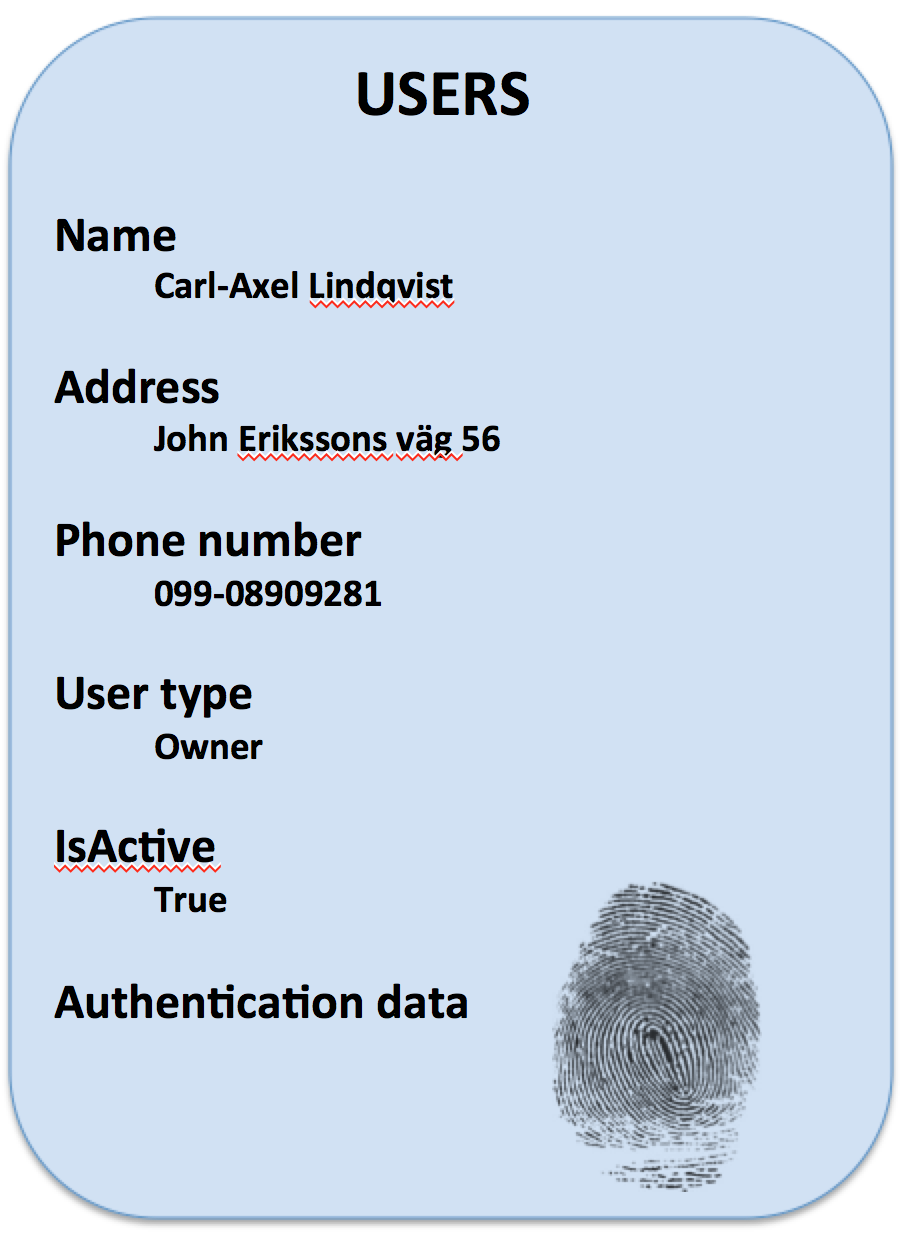
\includegraphics[width=0.6\textwidth]
    {VirtualWindow1.png}
  \caption{Virtual window that shows the data to be stored regarding users.}
  \label{vw1}
\end{figure}
      \subsubsection{Requirement}
\hfill \break 
\- \- \-The system must support the following user types:
\hfill \break 
\indent
\textbf{10.2.2.a} Passenger
\hfill \break 
\indent
\textbf{10.2.2.b} Driver
\hfill \break 
\indent
\textbf{10.2.2.c} Owner
\hfill \break 
\indent
\textbf{10.2.2.d} Admin
\todo{Kolla nummer}
      \subsubsection{Requirement}
\hfill \break 
\- \- \-There must be maximum one user with user type owner in the system
      \subsubsection{Requirement}
\hfill \break 
\- \- \-There must be one and only one user with user type admin in the system
      \subsubsection{Requirement}
\hfill \break 
\- \- \-The user type admin must have the name Admin
      \subsubsection{Requirement}
\hfill \break 
\- \- \-The system must store the user-entries according the data dictionary in figure DATA
\todo{krav}

\section{Manual Drive}



  \subsection{Activation}
\subsubsection {Requirement}
\hfill \break 
\- \- \-The following task must be supported by the system:\\
\hfill \break 
\textbf{Task:} \tab{User A attempts to drive the vehicle manually.}\\
\textbf{Purpose:} \tab{A requests to drive the vehicle manually.}\\
\textbf{Precondition:} \tab{The vehicle is not moving.}\\ 
\textbf{Trigger:} \tab{A selects manual mode via touchscreen or voice command.}\\
\\
\noindent
\textbf{Subtasks:} \tab{1.}    \tab{A attempts to authenticate.}\\
\tab{ } \tab{2.} \tab{A uses the breathalyser.}\\
\\
\noindent
\textbf{Variants:} \tab{1.}    \tab{A is authenticated and gains access to manual control}\\
\tab{ } \tab{ } \tab{mode.}\\
\tab{ } \tab{2a.} \tab{A is denied access due to lack of manual control}\\ \tab{ } \tab{ } \tab{permission.}\\
\tab{ } \tab{2b.} \tab{A is denied access due to recent alcohol consumption.}
\bigskip
  
  
      \subsubsection{Requirement}
\hfill \break 
\- \- \-The system must support manual driving of the car
      \subsubsection{Requirement}
\hfill \break 
\- \- \-It must be possible to request manual mode
      \subsubsection{Requirement}
\hfill \break 
\- \- \-9/10 new users authorized for manual driving must be able to request manual driving mode within 2 min
  \subsection{Personal safety}
      \subsubsection{Requirement}
\hfill \break 
\- \- \-For a passenger to be able to drive the car manually, the person must pass the blood alcohol content test
      \subsubsection{Requirement}
\hfill \break 
\- \- \-The blood alcohol content test has to be configured according to Swedish traffic law, which states that you are not allowed to drive with an alcohol level of 0.2 per mille or higher.
      \subsubsection{Requirement}
\hfill \break 
\- \- \-The blood alcohol content measuring device needs to be approved according to the european standard CENELEC 50436-1 and Swedish Transportstyrelsen regulation TSFS 2011:70
  \subsection{Road safety}
      \subsubsection{Requirement}
\hfill \break 
\- \- \-To turn on and off the automatic mode the car must be standing still
      \subsubsection{Requirement}
\hfill \break 
\- \- \-In order to initiate manual mode, the car must be standing still
      \subsubsection{Requirement}
\hfill \break 
\- \- \-When the system is in manual driving mode, the system must be active and avoid accidents the same way as in autonomous mode
      \subsubsection{Requirement}
\hfill \break 
\- \- \-The system must respond to a potential accident before the accident is unavoidable

\section{I/O}
\subsubsection {Requirement}
\hfill \break 
\- \- \-The following task must be supported by the system:\\
\hfill \break 
\textbf{Task:} \tab{User A instructs the car to drive to a destination.}\\
\textbf{Purpose:} \tab{Tell the system to drive from one place to another.}\\
\textbf{Precondition:} \tab{A is inside the vehicle and the doors are shut.}\\
\textbf{Trigger:} \tab{A gives a command to  CRASH.}\\
\\
\textbf{Variants:} \tab{1.} \tab{Command accepted, CRASH confirms the destination}\\
\tab{ } \tab{ } \tab{and drives A to the requested destination.}\\
\tab{ } \tab{2a.} \tab{Command rejected, the requested destination does not}\\ \tab{ } \tab{ } \tab{exist.}\\
\tab{ } \tab{2b.} \tab{Command rejected, no one in the car is}\\
\tab{ } \tab{ } \tab{authorized.}\\
\tab{ } \tab{2c.} \tab{Command rejected, CRASH has no GPS connection.}
\bigskip


    \subsubsection{Requirement}
\hfill \break 
\- \- \-When a command is entered feedback must be provided to the user
    \subsubsection{Requirement}
\hfill \break 
\- \- \-The system requires a network connection
    \subsubsection{Requirement}
\hfill \break 
\- \- \-A driver must be able to choose and change destination
  \subsection{Voice control}
      \subsubsection{Requirement}
\hfill \break 
\- \- \-The system requires a voice input device
      \subsubsection{Requirement}
\hfill \break 
\- \- \-The user must be able to interact with the system via voice controlled input
      \subsubsection{Requirement}
\hfill \break 
\- \- \-If the voice control system cannot interpret an incoming voice command, it must suggest to the user what it interpreted
      \subsubsection{Requirement}
\hfill \break 
\- \- \-7/10 times the voice control system must interpret the user command correctly
      \subsubsection{Requirement}
\hfill \break 
\- \- \-9/10 users must be able to select a route with the voice control system within 2 minutes
  \subsection{Touch screen}
      \subsubsection{Requirement}
\hfill \break 
\- \- \-The touch screen must have a touch precision more precise than 0.5 mm
      \subsubsection{Requirement}
\hfill \break 
\- \- \-The touch screen must have a resolution higher than 300 dots per inch
      \subsubsection{Requirement}
\hfill \break 
\- \- \-The touch screen must have a minimum size of 7 inches
      \subsubsection{Requirement}
\hfill \break 
\- \- \-9/10 users using the touch screen must be able to change the destination within 30 seconds
      \subsubsection{Requirement}
\hfill \break 
\- \- \-The touch screen shall support the design in figure \ref{fi:designmockup}.
\bigskip
\begin{figure}[htb]    
 \centering
  \includegraphics[width=0.9\textwidth]
    {"DesignReq".png}
  \caption{Design of the touch screen when a destination is set and the car is moving.}
  \label{fi:designmockup}
\end{figure}


\section{Remote}
\subsubsection {Requirement}
\hfill \break 
\- \- \-The following task must be supported by the system:\\
\hfill \break 
\textbf{Task:} \tab{User A remotely instructs the car to drive to a destination.}\\
\textbf{Purpose:} \tab{Request the system to drive from one place to another.}\\
\textbf{Precondition:} \tab{A is outside the vehicle and has remote access permissions via}\\
\tab{ } \tab{mobile device.}\\ 
\textbf{Trigger:} \tab{A starts the application on mobile device.}\\
\noindent
\\
\textbf{Subtasks:} \tab{1.} \tab{A authenticates to mobile device.}\\
\tab{ } \tab{2.} \tab{A specifies a destination}\\ 
%\tab{ } \tab{ } \tab{screen on mobile device.}\\
\\
\noindent
\textbf{Variants:} \tab{1a.}    \tab{A is granted access to mobile application and CRASH}\\
\tab{ } \tab{ } \tab{accepts the given command.}\\
\tab{ } \tab{1b.} \tab{A is granted access to mobile application but voice}\\ \tab{ } \tab{ } \tab{command is not accepted.}\\
\tab{ } \tab{2.} \tab{A is denied access to mobile application due to lack of}\\
\tab{ } \tab{ } \tab{remote access permission.} 
\bigskip

    \subsubsection{Requirement}
\hfill \break 
\- \- \-All commands that are available in the car must be available remotely
    \subsubsection{Requirement}
\hfill \break 
\- \- \-All commands that are available in the car must be available remotely
    \subsubsection{Requirement}
\hfill \break 
\- \- \-A user must be able to interact with the system remotely
    \subsubsection{Requirement}
\hfill \break 
\- \- \-The remote device must be able to display the last known location of the car

\section{Updates}
    \subsubsection{Requirement}
\hfill \break 
\- \- \-The system must be able to store future system updates
    \subsubsection{Requirement}
\hfill \break 
\- \- \-The system must be able to install stored future system updates at a given date
    \subsubsection{Requirement}
\hfill \break 
\- \- \-The system must query for new system updates once a day
    \subsubsection{Requirement}
\hfill \break 
\- \- \-System updates must only be performed when the car is parked

\section{Data storage}
    \subsubsection{Requirement}
\hfill \break 
\- \- \-The virtual windows must be supported by the system
    \subsubsection{Requirement}
\hfill \break 
\- \- \-The system must store route data
    \subsubsection{Requirement}
\hfill \break 
\- \- \-The system must store the following route data:
\hfill \break 
\indent
\textbf{15.0.16.a} Date
\hfill \break 
\indent
\textbf{15.0.16.b} Distance
\hfill \break 
\indent
\textbf{15.0.16.c} Estimated time to complete route
\hfill \break 
\indent
\textbf{15.0.16.d} Actual time to complete route
\hfill \break 
\indent
\textbf{15.0.16.e} Fuel consumption/km
\hfill \break 
\indent
\textbf{15.0.16.f} Total fuel consumption
\hfill \break 
\indent
\textbf{15.0.16.g} Name of the users in the car
\hfill \break 
\indent
\textbf{15.0.16.h} User type of the users in the car
\todo{Kolla nummer}


\section{Car Status}
  \subsection{Service log}
      \subsubsection{Requirement}
\hfill \break 
\- \- \-The system must store a service log
      \subsubsection{Requirement}
\hfill \break 
\- \- \- The system must store data corresponding to the virtual window concerning the service log
      \subsubsection{Requirement}
\hfill \break 
\- \- \-The service log must store the following data
\todo{Kolla nummer}
\hfill \break 
\indent
\textbf{15.1.3.a} Date
\hfill \break 
\indent
\textbf{15.1.3.b} Service type
\hfill \break 
\indent
\textbf{15.1.3.c} Service provider
\hfill \break 
\indent
\textbf{15.1.3.d} Mileage
\hfill \break 
\indent
\textbf{15.1.3.e} Optional description
      \subsubsection{Requirement}
\hfill \break 
\- \- \-The service log must contain the following data: date, repair nr, service provider, mileage, description
      \subsubsection{Requirement}
\hfill \break 
\- \- \-The system must store the service log-entries in the way described in figure 3
  \subsection{Status and service}
      \subsubsection{Requirement}
\hfill \break 
\- \- \-The system must notify the owner when the car needs a service
      \subsubsection{Requirement}
\hfill \break 
\- \- \-The car must be able to re-fuel on its own
      \subsubsection{Requirement}
\hfill \break 
\- \- \-The car must be able to re-fuel on its own

\section{Authentication}
\subsubsection {Requirement}
\hfill \break 
\- \- \-The following task must be supported by the system:\\
\hfill \break 
\textbf{Task:} \tab{Authenticate user A.}\\
\textbf{Purpose:} \tab{Authenticate A to retrieve user permissions.}\\
\textbf{Trigger:} \tab{User A tries to authenticate.}\\
\\
\noindent
\textbf{Variants:} \tab{1a.}    \tab{A is admin}\\
\tab{ } \tab{1b.} \tab{A is owner}\\
\tab{ } \tab{1c.} \tab{A is driver}\\
\tab{ } \tab{1d.} \tab{A is passenger with special permissions}\\
\tab{ } \tab{2.}  \tab{A is denied access}
\bigskip

    \subsubsection{Requirement}
\hfill \break 
\- \- \-The system requires an authentication sensor
    \subsubsection{Requirement}
\hfill \break 
\- \- \-The authentication sensor must have a margin of error less than 1 ppm


\section{Comfort}
    \subsubsection{Requirement}
\hfill \break 
\- \- \-The system must drive fuel efficiently
    \subsubsection{Requirement}
\hfill \break 
\- \- \-The ride must be comfortable for 9/10 users
    \subsubsection{Requirement}
\hfill \break 
\- \- \-EcoDriving must be performed according to the current definition by Sveriges Trafikskolors Riksförbund




\newpage




\begin{figure}[htb]    
 \centering
  \includegraphics[width=0.9\textwidth]
    {"Service log - VW".jpeg}
  \caption{Virtual window that shows the data to be stored regarding service logs.}
  \label{fig:Virtual window Service log}
\end{figure}
\newpage



\begin{thebibliography}{1}
\bibitem{srs} CRASH - Comfort, Reliability and Self Handling, Project Mission v2
\end{thebibliography}

\end{document}